\documentclass[11pt,a4paper]{article}
\usepackage[utf8]{inputenc}
\usepackage[T1]{fontenc}
\usepackage[brazil]{babel}
\usepackage{amsmath}
\usepackage{graphicx}
\usepackage{geometry}
\usepackage{float}
\geometry{margin=2.5cm}

\title{INF2608 -- Projeto 2: Algoritmo de Tracado de Caminhos}
\author{Lucca V. Rocha}
\date{30 de junho de 2026}

\begin{document}
\maketitle

\section{Resumo}

Este trabalho implementa um renderizador por tracado de caminhos em Python, usando NumPy para operacoes vetoriais e PIL para salvar imagens. A cena base e uma Cornell Box simples com paredes difusas, objetos geometricos e uma fonte de luz retangular no teto. O objetivo foi atender a aplicacao basica do enunciado, valendo 7 pontos, e acrescentar tres extensoes de 1 ponto: luz infinita, luz por poliedro triangular e MIS no ultimo trecho do caminho.

\section{Tecnicas adotadas}

O integrador implementado estima a equacao de transporte da luz:

\[
L_o(p,\omega_o) = L_e(p,\omega_o) +
\int_\Omega f_r(p,\omega_o,\omega_i)L_i(p,\omega_i)\cos\theta_i\,d\omega_i.
\]

A estimativa numerica usa Monte Carlo:

\[
F_N = \frac{1}{N}\sum_{i=1}^{N}\frac{f(X_i)}{p(X_i)}.
\]

Cada pixel e calculado pela media de varios caminhos independentes. Cada caminho acumula um fator de throughput. Em superficies difusas, a BRDF e constante:

\[
f_r = \frac{\rho}{\pi},
\]

onde $\rho$ e o albedo do material. As direcoes secundarias sao amostradas no hemisferio usando distribuicao ponderada pelo cosseno:

\[
p(\omega_i) = \frac{\cos\theta_i}{\pi}.
\]

Com essa escolha, o fator da continuacao difusa simplifica para o albedo, pois:

\[
\frac{(\rho/\pi)\cos\theta_i}{\cos\theta_i/\pi} = \rho.
\]

\section{Aplicacao basica}

A aplicacao basica foi implementada em \texttt{Trabalho 2/path\_tracer.py}. O codigo suporta esferas, caixas e planos; materiais difusos; superficies emissivas; fontes retangulares; multiplas amostras por pixel; profundidade maxima configuravel; jitter subpixel; correcao gamma; e cena base estilo Cornell Box.

A fonte retangular e amostrada uniformemente por area. Para calcular a contribuicao direta, o PDF de area e convertido para PDF de angulo solido:

\[
p_\omega = \frac{d^2}{\cos\theta_l A},
\]

onde $d$ e a distancia entre o ponto sombreado e a amostra na luz, $\theta_l$ e o angulo com a normal da luz, e $A$ e a area da fonte. Um raio de sombra e usado para descartar amostras ocluidas.

\begin{figure}[H]
\centering
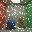
\includegraphics[width=0.42\linewidth]{img/base_cornell.png}
\caption{Cena base com Cornell Box, objetos difusos e fonte retangular.}
\end{figure}

\section{Comparacao de parametros}

A Figura~\ref{fig:spp} compara o efeito do numero de amostras por pixel. Com mais amostras, o ruido tende a diminuir porque a media de Monte Carlo converge para o valor esperado.

\begin{figure}[H]
\centering
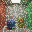
\includegraphics[width=0.30\linewidth]{img/spp_16.png}
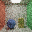
\includegraphics[width=0.30\linewidth]{img/spp_64.png}

\includegraphics[width=0.30\linewidth]{img/spp_256.png}
\caption{Comparacao de 16, 64 e 256 amostras por pixel.}
\label{fig:spp}
\end{figure}

A Figura~\ref{fig:depth} compara profundidades 2, 4 e 6. A profundidade 4 e a configuracao minima exigida para a entrega principal. Profundidades maiores permitem mais interreflexoes difusas, mas aumentam o custo.

\begin{figure}[H]
\centering
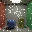
\includegraphics[width=0.30\linewidth]{img/depth_2.png}
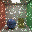
\includegraphics[width=0.30\linewidth]{img/depth_4.png}
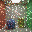
\includegraphics[width=0.30\linewidth]{img/depth_6.png}
\caption{Comparacao de profundidade maxima 2, 4 e 6.}
\label{fig:depth}
\end{figure}

\section{Extensao 1: luz infinita}

A luz infinita representa radiancia vinda do ambiente. Quando um raio nao intersecta nenhum objeto, o renderizador retorna uma cor de ambiente dependente da direcao. Para tornar o efeito visivel, foi criada uma cena parcialmente aberta, permitindo que raios escapem da caixa.

\begin{figure}[H]
\centering
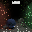
\includegraphics[width=0.42\linewidth]{img/environment_light.png}
\caption{Cena aberta iluminada tambem por luz infinita do ambiente.}
\end{figure}

\section{Extensao 2: luz por poliedro}

A fonte poliedrica e representada por uma malha de triangulos emissivos. Cada triangulo tem area:

\[
A_t = \frac{1}{2}\|(b-a)\times(c-a)\|.
\]

A amostragem escolhe um triangulo com probabilidade proporcional a sua area e depois amostra um ponto uniforme usando coordenadas baricentricas:

\[
r_1=\sqrt{\xi_1},\quad
p=(1-r_1)a+r_1(1-\xi_2)b+r_1\xi_2c.
\]

O PDF total de area e $1/A_{total}$. Na demonstracao, foi usado um tetraedro emissivo.

\begin{figure}[H]
\centering
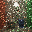
\includegraphics[width=0.42\linewidth]{img/mesh_light.png}
\caption{Iluminacao por fonte poliedrica triangulada.}
\end{figure}

\section{Extensao 3: MIS no ultimo trecho}

O MIS combina duas estrategias para estimar a conexao final com a luz:

\begin{enumerate}
\item amostragem explicita da fonte;
\item amostragem pela BRDF difusa.
\end{enumerate}

As PDFs sao comparadas no dominio de angulo solido. O peso usa a heuristica balanceada:

\[
w_i = \frac{p_i}{p_1+p_2}.
\]

Assim, uma amostra da fonte recebe peso:

\[
w_l = \frac{p_l}{p_l+p_b},
\]

e uma amostra da BRDF recebe peso:

\[
w_b = \frac{p_b}{p_l+p_b}.
\]

A cena de comparacao usa uma fonte menor, que tende a evidenciar o ruido quando a BRDF raramente acerta a luz.

\begin{figure}[H]
\centering
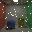
\includegraphics[width=0.42\linewidth]{img/mis_off.png}
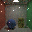
\includegraphics[width=0.42\linewidth]{img/mis_on.png}
\caption{Comparacao sem MIS e com MIS para uma fonte pequena.}
\end{figure}

\section{Analise dos resultados}

O renderizador mostra o comportamento esperado de um path tracer: imagens com poucas amostras sao ruidosas, enquanto mais amostras reduzem a variancia. O aumento da profundidade permite que a luz se espalhe por mais rebatimentos difusos, mas tambem aumenta o tempo de renderizacao. A luz infinita e simples e isolada, pois afeta apenas raios sem intersecao. A luz poliedrica reaproveita a mesma logica de amostragem por area usada na luz retangular. O MIS melhora a estimativa do ultimo trecho ao combinar amostras da fonte e da BRDF com pesos baseados nos PDFs.

\section{Como executar}

Render basico:

\begin{verbatim}
python3 "Trabalho 2/path_tracer.py" --scene base_cornell \
  --width 160 --height 160 --spp 16 --depth 4 \
  --output "Trabalho 2/img/base_cornell.png"
\end{verbatim}

Gerar o conjunto de imagens do relatorio:

\begin{verbatim}
python3 "Trabalho 2/path_tracer.py" --scene all \
  --width 160 --height 160 --spp 16 --depth 4 \
  --output-dir "Trabalho 2/img"
\end{verbatim}

\end{document}
